Im Versuch werden die Übergänge des Cadmiums unter Aufspaltung durch den Zeeman-Effekt betrachtet.
Dem roten Licht liegt dabei der normale Zeeman-Effekt zugrunde, dem blauen Licht der anormale Zeeman-Effekt.\\
Die Orientierungsquantenzahl $m$ ergibt sich für den normalen Zeeman-Effekt (rot) zu
\begin{equation*}
  m_{\text{exp}} = \SI{0.724 \pm 0.012}{},
\end{equation*}
was mit einer relativen Abweichung von $f=\SI{27.6}{\%}$ zur theoretischen Quantenzahl
\begin{equation*}
  m_{\text{theo}} = \SI{1}{}
\end{equation*}
des zirkularen Übergangs passt.
\begin{figure}[h!]
  \centering
  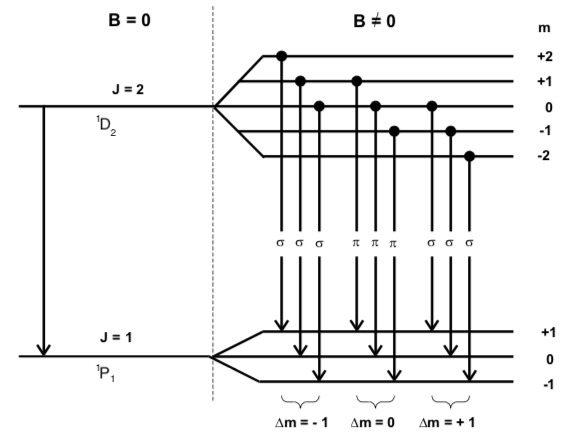
\includegraphics[width=\textwidth]{normal.png}
  \caption{Aufspaltung durch den normalen Zeeman-Effekt \cite{1}}
  \label{fig:normal}
\end{figure}
\FloatBarrier
Für die Übergänge des anormalen Zeeman-Effekts werden die Landé-Faktoren des Übergangs $g_{ij}=m_{1}g_{1}-m_{2}g_{2}$ berechnet und mit der Theorie verglichen.
\begin{align*}
  \text{zirkular}  &&& g_{ij, \text{exp}} &= \SI{1.30 \pm 0.02}{}    &&&   g_{ij, \text{theo}} &= \SI{2}{}     &&&  f=\SI{35.0}{\%}   \\
  \text{linear}    &&& g_{ij, \text{exp}} &= \SI{0.442 \pm 0.004}{}  &&&   g_{ij, \text{theo}} &= \SI{0.5}{}   &&&  f=\SI{11.6}{\%}   .
\end{align*}
\begin{figure}[h!]
  \centering
  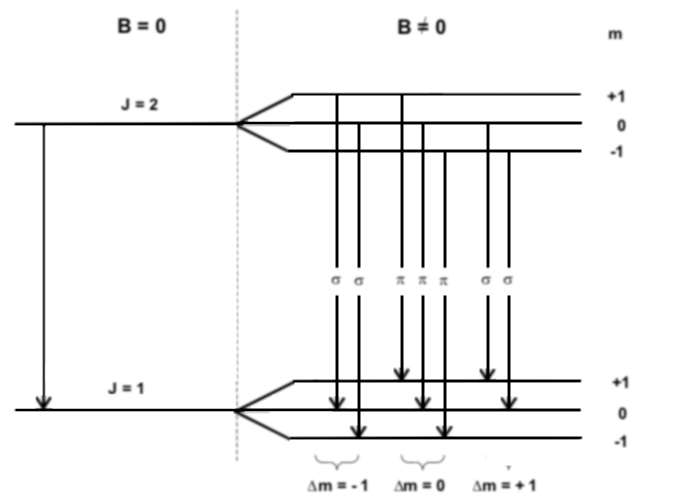
\includegraphics[width=\textwidth]{anormal.png}
  \caption{Aufspaltung durch den anormalen Zeeman-Effekt \cite{1}}
  \label{fig:normal}
\end{figure}
